%
% File acl2012.tex
%
% Contact: Maggie Li (cswjli@comp.polyu.edu.hk), Michael White (mwhite@ling.osu.edu)
%%
%% Based on the style files for ACL2008 by Joakim Nivre and Noah Smith
%% and that of ACL2010 by Jing-Shin Chang and Philipp Koehn


\documentclass[11pt,letterpaper]{article}
\usepackage[letterpaper]{geometry}
\usepackage{acl2012}
\usepackage{times}
\usepackage{latexsym}
\usepackage{amsmath}
\usepackage{multirow}
\usepackage{graphicx}
\usepackage{todonotes}
\usepackage{url}
\usepackage{color}
\usepackage[inline]{enumitem}
\usepackage[]{caption}
\usepackage{subcaption}
\usepackage{tikz}
\usetikzlibrary{shapes.geometric}
\makeatletter
\newcommand{\@BIBLABEL}{\@emptybiblabel}
\newcommand{\@emptybiblabel}[1]{}
\makeatother
\usepackage[hidelinks]{hyperref}
\DeclareMathOperator*{\argmax}{arg\,max}

\newcommand{\term}{\textit}

\newcommand{\Listener}{L}
\newcommand{\Speaker}{S}
\newcommand{\utt}{u}
\newcommand{\uttlen}{N}
\newcommand{\referent}{c}
\newcommand{\context}{C}
\newcommand{\contextlen}{K}
\newcommand{\target}{t}
\newcommand{\numsamples}{m}
\newcommand{\feat}{f}
\renewcommand{\|}{\mid}
\newcommand{\best}[1]{\textbf{#1}}
\newcommand{\oracle}[1]{\textit{#1}}

\newcommand{\Secref}[1]{Section~\ref{#1}}
\newcommand{\secref}[1]{Section~\ref{#1}}
\newcommand{\dashsecref}[2]{Sections~\ref{#1}--\ref{#2}}
\newcommand{\Figref}[1]{Figure~\ref{#1}}
\newcommand{\figref}[1]{Figure~\ref{#1}}
\newcommand{\dashfigref}[2]{Figures~\ref{#1}--\ref{#2}}
\newcommand{\Tabref}[1]{Table~\ref{#1}}
\newcommand{\tabref}[1]{Table~\ref{#1}}
\newcommand{\pararef}[1]{\textbf{#1}}

\definecolor{ourlightblue}{HTML}{03A9F4}
\definecolor{ourgreen}{HTML}{4D8951}
\definecolor{oursteelblue}{HTML}{9BB8D7}
\definecolor{ourorange}{HTML}{FDBA58}

\newcommand{\ourlightblue}[1]{{\color{ourlightblue}#1}}
\newcommand{\ourgreen}[1]{{\color{ourgreen}#1}}
\newcommand{\oursteelblue}[1]{{\color{oursteelblue}#1}}
\newcommand{\ourorange}[1]{{\color{ourorange}#1}}

\newcommand{\todocheck}[1]{\textcolor{red}{#1}}

\setlength\titlebox{6.5cm}    % Expanding the titlebox

\title{Colors in Context: A Pragmatic Neural Model for \\
Grounded Language Understanding}

% \author{First Author \\
%   Affiliation / Address line 1 \\
%   Affiliation / Address line 2 \\
%   Affiliation / Address line 3 \\
%   {\tt email@domain} \\\And
%   Second Author \\
%   Affiliation / Address line 1 \\
%   Affiliation / Address line 2 \\
%   Affiliation / Address line 3 \\
%   {\tt email@domain} \\}

\date{}

\begin{document}
\maketitle
\begin{abstract}


We present a two-layer pragmatic model of referring expression interpretation:
a listener modeling a speaker modeling a listener, where the base listener is a
recurrent neural network classifier. Our model outperforms the
base listener at a task of color reference understanding, evaluated on a
newly-collected corpus of human utterances in color reference games.
Our experiments show that the primary benefits from pragmatic reasoning come
in the hardest cases: when the model must distinguish colors that are very
similar, or when there are few utterances available that adequately express
the target color.

\end{abstract}

\section{Introduction}

Grounded language use requires adapting language to the context at hand: trying
to identify an object by describing it as ``blue'' will be unhelpful if all
accessible objects are some shade of blue. People assume their interlocutors know
this and adapt their interpretation of grounded language accordingly. This intuition
is captured in game-theoretic and probabilistic models of pragmatic
language understanding \cite{Jaeger2012,Frank2012}.

In this paper, we present a model of pragmatic interpretation that combines a
recurrent neural network model of color description understanding
\cite{MonroeGoodmanPotts16_Color} with a
Bayesian formalization of pragmatic reasoning through embedded agent modeling
\cite{Goodman2013}.

We evaluate our model in a \term{reference game} task: given a context consisting
of a set of potential \term{referents}, one referent is selected as the \term{target}
and its identity indicated secretly to the \term{speaker}. The speaker then must
convey the identity of the target to a \term{listener}. Our model plays the
role of the listener in this game, attempting to resolve a human utterance
to the correct referent. The reference game setting tests the ability of our model
to do two distinct forms of pragmatic reasoning: the model must consider
not only world context in the form of the set of available referents,
but also linguistic context in the form of the speaker's goals and constraints in 
describing the target.

This paper presents a new corpus of reference games in which the referents
are patches of color. The corpus includes 942 complete games with
47,100 utterances produced by humans playing these games with real-time
feedback. We focus on color because color perception exhibits many
cognitively-interesting properties, and understanding of color descriptions
requires understanding many of the intricacies of language in
general---compositionality, vagueness, etc.---despite the fact that
color is a fundamentally low-dimensional space.
While many datasets exist featuring descriptions of individual colors 
\cite{Cook2005,Munroe2010,Kawakami2016}, situating colors in context
elicits much greater variety in language use, including negations,
comparatives and superlatives, and increased use of
metaphor and shared associations.

Experiments on this data show that our pragmatic model improves accuracy
in interpreting human-produced descriptions over the RNN-based classifier
alone. Moreover, the improvements from pragmatic reasoning come primarily
in the hardest cases. By this we mean \begin{enumerate*}[label=(\arabic*)]
\item contexts featuring colors that are very similar, thus
requiring the interpretation of descriptions that convey fine distinctions; and
\item target colors that most referring expressions fail to identify, whether
due to a lack of adequate descriptive terms or a consistent bias against the
color in the RNN listener.
\end{enumerate*}

\section{Task and data collection}

We compare agents on a task of language understanding in a reference game. An agent $\Listener$ is presented with a list of colors $\context = \{\referent_i, i=1..\contextlen\}$ and an utterance $\utt$ that describes the target color $\referent_\target \in \context$ in natural language. The agent does not know the index $\target$ of the target color and must guess it from $\utt$.

To collect a corpus of natural color reference data across varying contexts, we recruited \todocheck{\#} unique participants from Amazon Mechanical Turk to play 1,117 real-time, multi-player communication games of 50 rounds each \cite{Hawkins15_RealTimeWebExperiments}. \todocheck{After non-native english speakers and incomplete games were excluded, we were left with a corpus of 47,100 utterances across 942 games [report modal number of games per turker?]}. Participants were sorted into dyads, assigned the role of speaker or listener, and placed in a game environment containing a chat box and an array of three color patches (\figref{fig:taskScreenshot}).

\begin{figure}
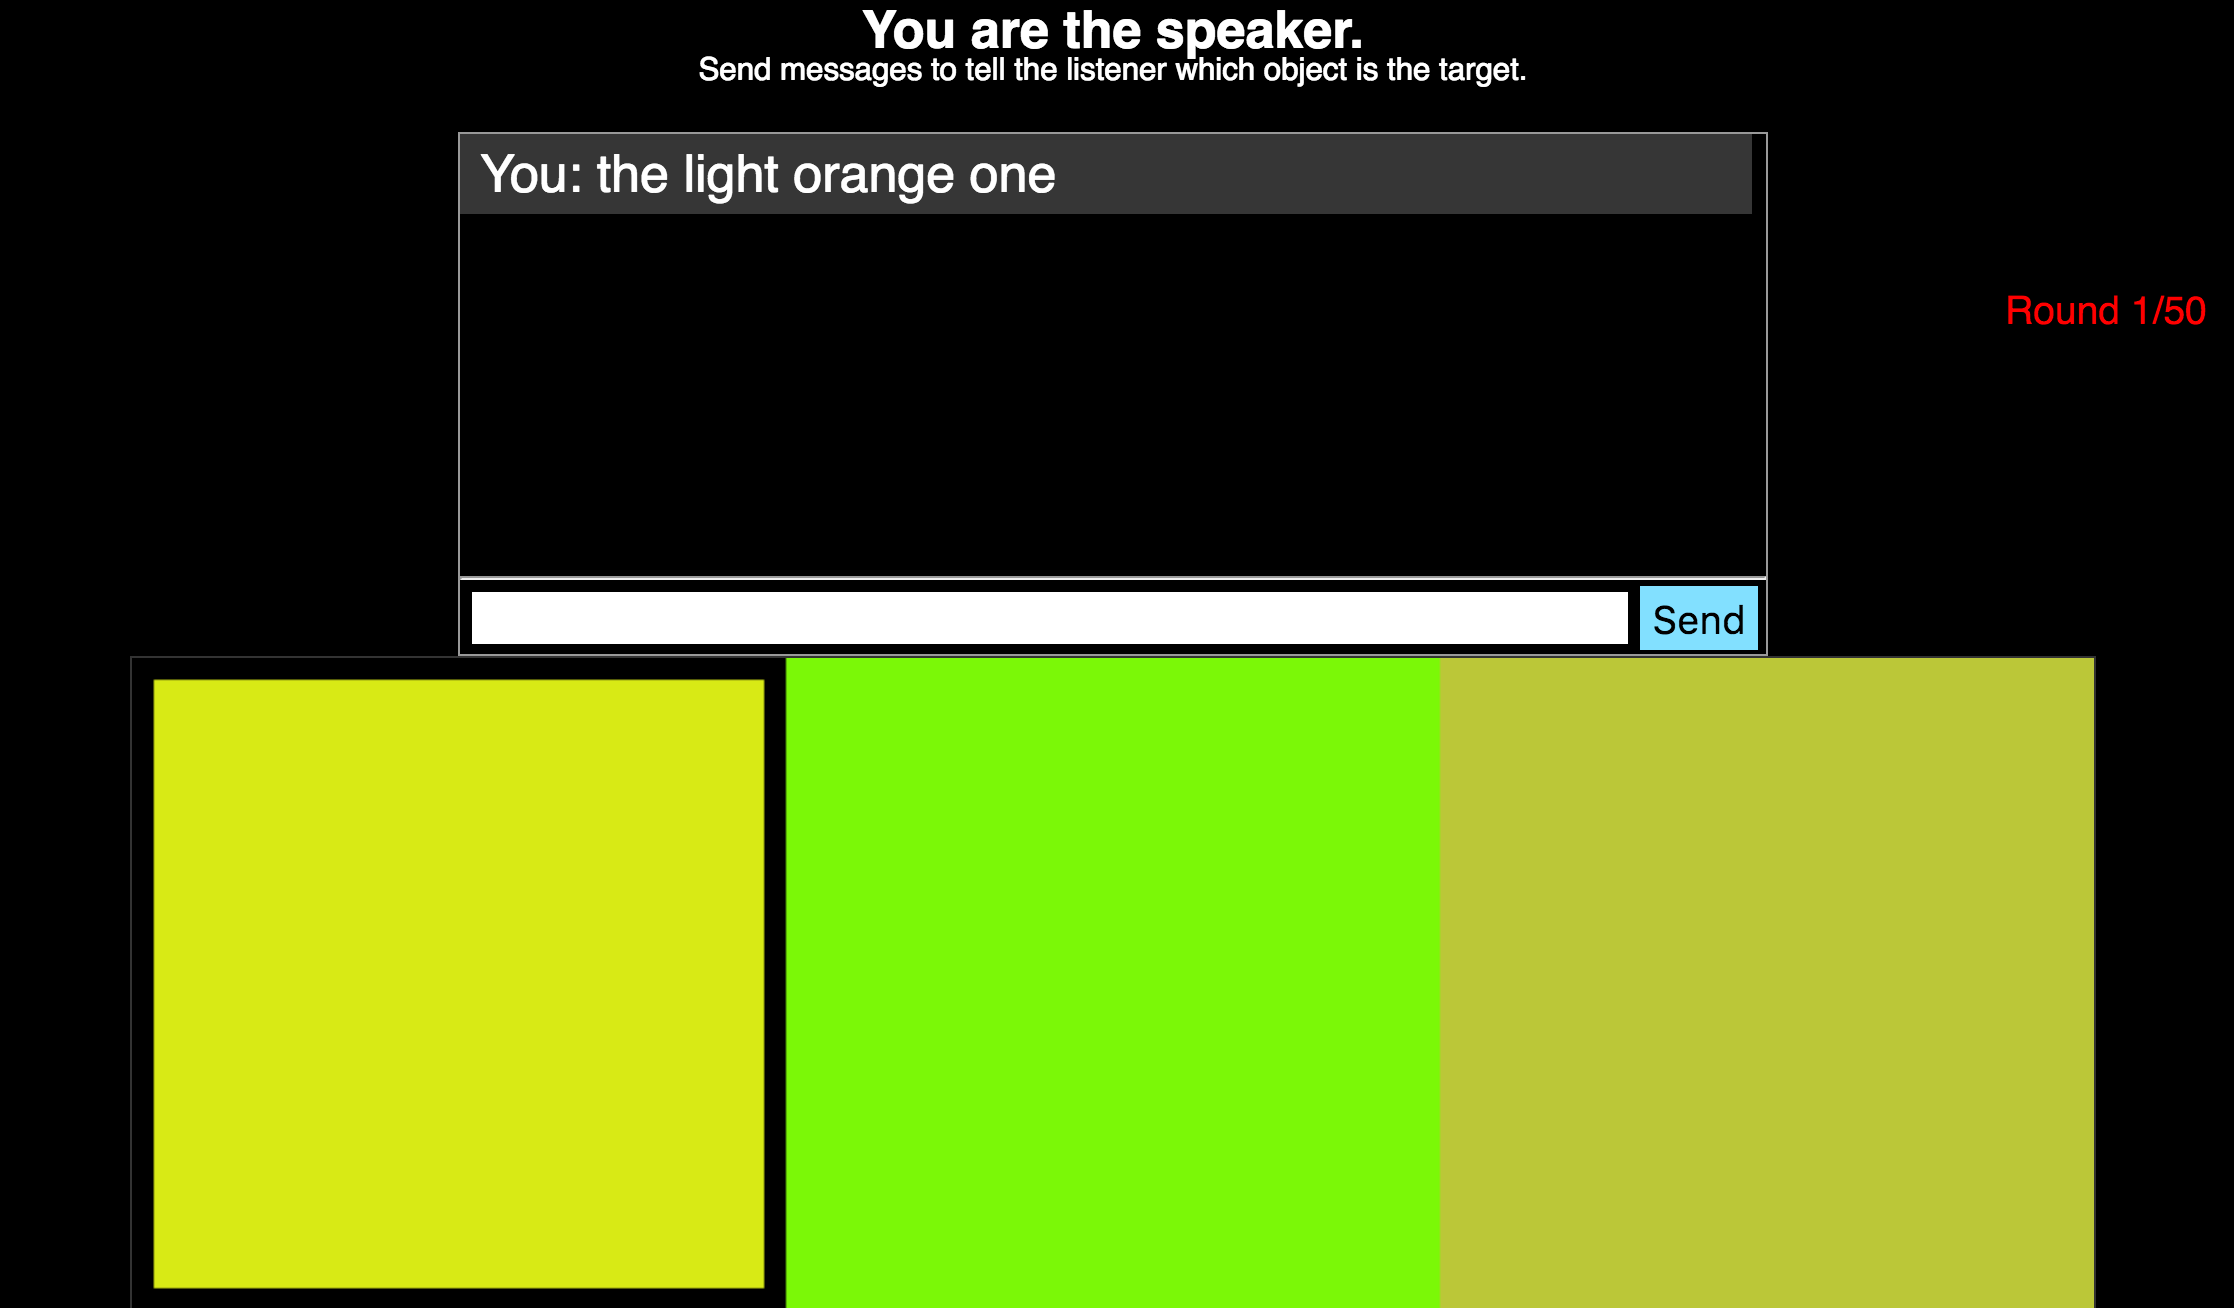
\includegraphics[scale = .2]{figures/speakerView.png}
\caption{Example trial in corpus collection task, from speaker's perspective}
\label{fig:taskScreenshot}
\end{figure}

On each round, one of the three colors was chosen to be the ``target'' and highlighted for the speaker. They were instructed to communicate this information to the listener, who could then click on one of the colors to advance to the next trial. Both participants were free to use the chat box at any point during the trial. 

To ensure a range of difficulty, we randomly interspersed an equal number of trials from three different conditions: (1) \emph{close}, where colors were all within a distance of $\theta$ from one another but still perceptible\footnote{We used the most recent CIEDE standard to measure color differences, which is calibrated to human vision \cite{SharmaWuDalal05_DeltaE}. All distances were constrained to be larger than a lower bound of $\epsilon = 5$ to ensure perceptible differences, and we used a threshold value of $\theta = 20$ to create conditions}, (2) \emph{split}, where one distractor was within a distance of $\theta$ of the target, but the other distractor was further than $\theta$, and (3) \emph{far}, where all colors were farther than $\theta$ from one another. Colors were rejection sampled uniformly from RGB (red, green, blue) space to meet these constraints. 

\section{Models}

Our model consists of a recurrent neural network (RNN)--based speaker and listener 
embedded within a higher-order reasoning listener. \todocheck{(intro to RSA here)}

\begin{figure*}[t]
  \centering
  \begin{subfigure}[b]{0.48\textwidth}
    \footnotesize
\centering
\begin{tikzpicture}[scale=0.90]

  \tikzstyle{label}=[anchor=east,align=right,text width=2.5cm]
  \tikzstyle{colorvec}=[draw, minimum width=6mm, minimum height=4mm]
  \tikzstyle{hiddencolorvec}=[draw, minimum width=6mm, minimum height=4mm]
  \tikzstyle{token}=[draw]
  \tikzstyle{LSTM}=[draw,circle, minimum width=6mm, minimum height=4mm]
  \tikzstyle{FC}=[draw, minimum width=1cm, minimum height=0.4cm]
  \tikzstyle{softmax}=[draw,isosceles triangle,rotate=90]
  \tikzstyle{output}=[inner sep=0]

  \path
  (1,0) node[colorvec,fill=ourlightblue](cx){$c_{1}$}
  (2.5,0) node[colorvec,fill=ourgreen](cy){$c_{2}$}
  (4,0) node[colorvec,fill=oursteelblue](cz){$c_{t}$};

  \path
  (1, 1) node[LSTM](hx){}
  (2.5, 1) node[LSTM](hy){}
  (4, 1) node[LSTM](hz){$h$};

  \path
  (5.5, 1) node[token](tx){$h;\langle s\rangle$}
  (7, 1) node[token](ty){$h; u_{1}$}
  (8.5,1) node[token](tz){$h; u_{2}$};

  \path
  (5.5, 2) node[LSTM](lx){}
  (7, 2) node[LSTM](ly){}
  (8.5,2) node[LSTM](lz){};

  \path
  (5.5, 3) node[FC](fx){}
  (7, 3) node[FC](fy){}
  (8.5,3) node[FC](fz){};

  \path
  (5.5, 4) node[softmax](sx){}
  (7, 4) node[softmax](sy){}
  (8.5,4) node[softmax](sz){};

  \path
  (5.5, 5) node[output](yx){$u_{1}$}
  (7, 5) node[output](yy){$u_{2}$}
  (8.5,5) node[output](yz){$\langle/s\rangle$};

  \draw (4.75,2) node[label]{LSTM};
  \draw (4.75,3) node[label]{Fully connected};
  \draw (4.75,4) node[label]{Softmax};

  \draw (cx)--(hx);
  \draw (cy)--(hy);
  \draw (cz)--(hz);

  \draw (hx)--(hy)--(hz);
  \draw (lx)--(ly)--(lz);

  \draw (tx)--(lx)--(fx)--(sx)--(yx);
  \draw (ty)--(ly)--(fy)--(sy)--(yy);
  \draw (tz)--(lz)--(fz)--(sz)--(yz);

  \draw[->,draw=ourgreen] (hz) to[out=-45,in=225] (tx);
  \draw[->,draw=ourgreen] (hz) to[out=-45,in=225] (ty);
  \draw[->,draw=ourgreen] (hz) to[out=-45,in=225] (tz);

  \draw[->,draw=ourorange] (yx) to[out=10,in=140] (ty);
  \draw[->,draw=ourorange] (yy) to[out=10,in=140] (tz);
\end{tikzpicture}

    \caption{The $\Speaker_{0}$ agent processes the target color
      $c_{T}$ in context and produces a color description
      sequentially. Each step in production is conditioned by the
      final contextual representation $h$ and the previous word
      produced.}
  \end{subfigure}
  \hfill
  \begin{subfigure}[b]{0.48\textwidth}
    \footnotesize
\centering
\begin{tikzpicture}[scale=0.90]

  \tikzstyle{wordvec}=[draw, minimum width=6mm, minimum height=4mm]
  \tikzstyle{embedding}=[draw, minimum width=6mm, minimum height=4mm]
  \tikzstyle{LSTM}=[draw,circle, minimum width=6mm, minimum height=4mm]
  \tikzstyle{linear}=[draw, minimum width=1.5cm, minimum height=4mm]
  \tikzstyle{dist}=[draw, minimum width=1.5cm, minimum height=4mm]
  \tikzstyle{score}=[inner sep=0pt]
  \tikzstyle{softmax}=[draw,
                       isosceles triangle,
                       rotate=90,
                       top color=oursteelblue,
                       bottom color=ourgreen,
                       minimum size=8mm]
  \tikzstyle{colorvec}=[draw, minimum width=6mm, minimum height=4mm]
  \tikzstyle{output}=[draw]

  \tikzstyle{label}=[align=left,text width=2cm]

  \path
  (1,  0) node[wordvec](xx){$x_{1}$}
  (2.5,0) node[wordvec](xy){$x_{2}$}
  (4,  0) node[wordvec](xz){$x_{3}$};

  \path
  (1,  1) node[embedding](hx){}
  (2.5,1) node[embedding](hy){}
  (4,  1) node[embedding](hz){};

  \path
  (1,  2) node[LSTM](lx){}
  (2.5,2) node[LSTM](ly){}
  (4,  2) node[LSTM](lz){};

  \path
  (4, 3) node[linear](linx){$(\mu, \Sigma)$};

  \path
  (6,3) node[colorvec,fill=ourlightblue](cx){$c_{1}$}
  (7,3) node[colorvec,fill=ourgreen](cy){$c_{2}$}
  (8,3) node[colorvec,fill=oursteelblue](cz){$c_{3}$};

  \path
  (4, 4) node[dist](scores){}
  (3.5, 4) node[score](scorex){$\bullet$}
  (4, 4) node[score](scorey){$\bullet$}
  (4.5, 4) node[score](scorez){$\bullet$};

  \path
  (4, 5) node[softmax](sx){};

  \path
  (4, 6) node[output,fill=oursteelblue](yx){$c_{3}$};

  \draw (6, 1) node[label]{Embedding};
  \draw (6, 2) node[label]{LSTM};
  %\draw (6, 3) node[label]{Linear transform};
  \draw (6, 5) node[label]{Softmax};

  \draw (lx)--(ly)--(lz);
  \draw (xx)--(hx)--(lx);
  \draw (xy)--(hy)--(ly);
  \draw (xz)--(hz)--(lz)--(linx)--(scores)--(sx)--(yx);


  \draw[draw=ourgreen] (cx) to[out=120,in=300] (scorex);
  \draw[draw=ourgreen] (cy) to[out=120,in=320] (scorey);
  \draw[draw=ourgreen] (cz)  to[out=120,in=340] (scorez);

  \draw (linx)--(scorex);
  \draw (linx)--(scorey);
  \draw (linx)--(scorez);

\end{tikzpicture}

    \caption{The $\Listener_{0}$ agent processes a color description
      sequentially. The final represententation is transformed into a
      Gaussian distribution in color space, which is used to score the
      context colors.}
  \end{subfigure}
  \caption{The neural base speaker and listener agents.
    \todocheck{RNN initial states not shown. Seem okay?}}
  \label{fig:model}
\end{figure*}

\subsection{Representing colors}

Each color is represented in its simplest form as a three-dimensional vector in
RGB space; our models transform this to HSV (hue, saturation,
value) as a preprocessing step.

The vectors that are used as input to the RNN models are Fourier-transformed as in \newcite{MonroeGoodmanPotts16_Color}:
a color
$(h, s, v)$ is mapped to a higher-dimensional\footnote{For the listener, we restrict $j,k$ to $\{0, 1\}$ and $\ell$ to 0, as we
found this improved performance slightly.} vector $\feat$:
\begin{align*}
\hat{\feat}_{jk\ell} &= \exp \left[-2\pi i \left(jh^* + ks^* + \ell v^*\right)\right] \\
\feat &= \begin{bmatrix}
  \Re{\hat{\feat}} & \Im{\hat{\feat}}
\end{bmatrix}\qquad j,k,\ell \in \{0,1,2\} 
\end{align*}
where $(h^*, s^*, v^*) = (h / 360, s / 200, v/200)$.
The Fourier transformation is meant to help the models identify non-convex components
of denotations of color language, particularly periodic components.

\subsection{Classifier listener}

Our base listener agent $\Listener_0$ is an LSTM encoder model that produces a Gaussian
distribution over colors in a transformed representation space.

The words in the input are embedded in a 100-dimensional vector space. Word embeddings
are initialized randomly \todocheck{(how?)} and trained. The sequence of word vectors are
used as input to an LSTM with 100-dimensional hidden state, and a linear
transformation is applied to the output representation to produce a covariance matrix
and mean vector for a Gaussian distribution in color representation space. 
The Gaussian scores for each of the $\contextlen$ context colors are normalized to
produce a probability distribution over the context colors. We denote this probability
distribution by $\Listener_0(\target \| \utt, \context; \theta)$, where $\theta$ represents the
vector of parameters that define the trained model.
\todocheck{(reference listener figure)}

\subsection{Classifier speaker}\label{sec:s0}

In order to avoid enumerating an exponentially large space of possible utterances,
we also employ a probabilistic speaker model
$\Speaker_0(\utt \| \target, \context; \phi)$ to generate sets of alternative
utterances for each context.

The speaker model consists of an LSTM context encoder
and an LSTM description decoder. In this model, the colors of the context
$\referent_i \in \context$ are transformed into Fourier representation space,
and the sequence of color representations is passed through an LSTM with
100-dimensional hidden state.

The output of this recurrent neural network is concatenated with a
100-dimensional embedding for the previous token at each time step in decoding.
The resulting vector is input along with the previous cell state to the LSTM cell,
and an affine transformation and softmax function are applied to the output to
produce a probability distribution predicting the following token of the description.
\todocheck{(reference speaker figure)}

\subsection{Pragmatic listener}

From the base classifier listener, we build a listener agent that performs
pragmatic inference using an embedded speaker model. This agent is based on the
pragmatic listener of \newcite{Goodman2013}, denoted
$\Listener(\Speaker(\Listener_0))$: a listener modeling a speaker modeling the
base listener.

Formally, our pragmatic listener $\Listener_2$ is defined in terms of the base
listener as follows:
\begin{align}
\Speaker_1(\utt \| \target, \context; \theta) &= \frac{\Listener_0(\target \| \utt, \context; \theta)^\alpha}{\sum_{\utt'} \Listener_0(\target \| \utt', \context; \theta)^\alpha} \label{eq:s1} \\
\Listener_2(\target \| \utt, \context; \theta) &= \frac{\Speaker_1(\utt \| \target, \context; \theta)}{\sum_{\target'} \Speaker_1(\utt \| \target', \context; \theta)} \nonumber
\end{align}

Theoretically, the denominator in \eqref{eq:s1} should consist of a sum over
the entire set of potential utterances, which is exponentially large in the
maximum utterance length. As mentioned in \secref{sec:s0}, we limit this search by
taking $\numsamples = 8$ samples from $\Speaker_0(\utt \| i, \context; \phi)$ for
each possible target index $i$, adding the actual utterance from the testing example,
and taking the resulting set as the universe of possible utterances. Taking a number
of samples from $\Speaker_0$ for each referent in the context gives the pragmatic
listener a variety of informative alternative utterances to consider when
interpreting the true input description.

The \term{inverse temperature} parameter $\alpha$ governs the ``rationality'' of
the speaker modeled by the pragmatic listener; a large $\alpha$ means that the
listener expects the speaker to choose the most informative utterance consistently, 
whereas a small $\alpha$ means the listener expects the speaker to choose suboptimal
utterances frequently. This affects the listener's interpretations: the more reliable
the speaker is in choosing the optimal utterance for a referent, the more the
listener will take deviations from an optimal utterance as a signal to choose a
different referent.

We find we can obtain an additional small improvement in listener accuracy
by blending the pragmatic listener with the base listener:
\begin{align}
\Listener^{*}(\target \| \utt, \context; \theta) &\propto {\Listener_0}(\target \| \utt, \context; \theta)^{\beta} \cdot {} \nonumber \\
&\phantom{{} \propto {}} \Listener_2(\target \| \utt, \context; \theta)^{1-\beta}  \label{eq:beta}
\end{align}

This allows the model to adjust the extent to which it overrides the learned model
with the pragmatic reasoning. A base weight $\beta = 0$ makes the blended model
equivalent to the pragmatic model, and $\beta = 1$ ignores the pragmatic reasoning
and uses the base model's outputs.

\subsection{Training} \label{sec:training}

Our listener and speaker models are trained using Adadelta \todocheck{(cite)} and
Adam \todocheck{(cite)}, adaptive variants of stochastic gradient descent (SGD).
The choice of optimization algorithm and learning rate for each model\footnote{For
$\Speaker_0$: Adam, learning rate $\alpha = {}$0.004; for $\Listener_0$: Adadelta,
learning rate $\eta = {}$0.2.}
were tuned with grid search on a held-out tuning set consisting of 3,500 contexts.

We also use a more fine-grained grid search on this tuning set to determine the
values of the two pragmatic reasoning parameters, $\alpha$ and $\beta$.
Our final model uses
$\alpha = 0.544$ and $\beta = -0.15$; see \secref{sec:alpha_beta} for more
discussion of these values.

% latex table generated in R 3.3.0 by xtable 1.8-2 package
% Thu Nov 17 15:41:24 2016
\begin{table*}[ht]
\centering
\begin{tabular}{lrrr|rrr}
  & \multicolumn{3}{c}{human}& \multicolumn{3}{c}{model}\\ \hline
  & far& split& close& far& split& close\\ \hline
\# Chars & 7.53 & 11.30 & 12.93 & 8.51 & 11.60 & 14.31 \\ 
  \# Comparatives & 0.02 & 0.14 & 0.13 & 0.04 & 0.09 & 0.13 \\ 
  \# Negatives & 0.03 & 0.10 & 0.12 & 0.05 & 0.09 & 0.13 \\ 
  \# Superlatives & 0.02 & 0.06 & 0.16 & 0.05 & 0.10 & 0.17 \\ 
  \# Words & 1.46 & 2.04 & 2.27 & 1.61 & 2.09 & 2.51 \\ 
   \hline
\end{tabular}
\caption{Corpus statistics and statistics of samples from $\Speaker_1$ (rates per utterance). \todocheck{todo: put errors in, include wordnet level of informativity}} \label{table:metrics}
\end{table*}


\section{Behavioral results}

\begin{figure}
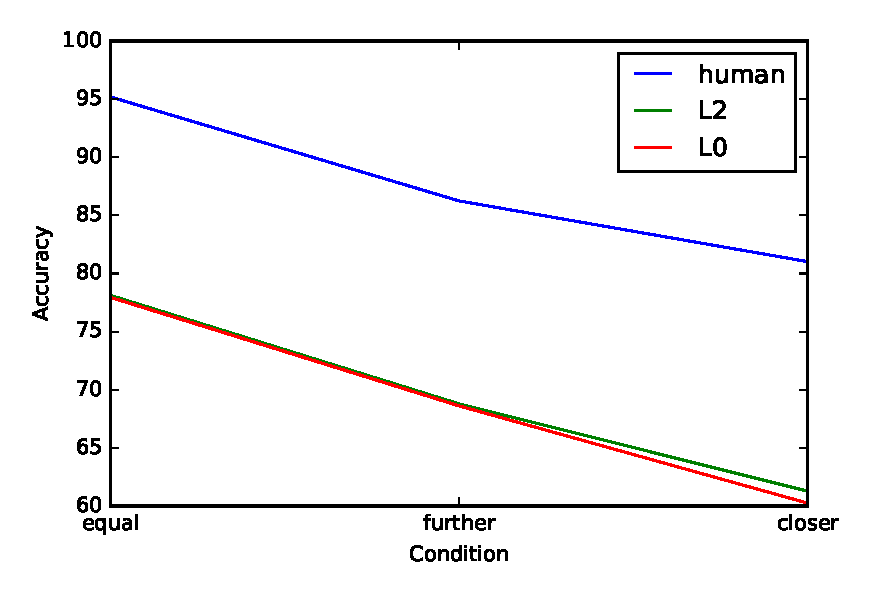
\includegraphics[scale = .5]{figures/allListenerAccuracy.eps}
\caption{Listener performance across conditions, for both human participants and model output}
\label{fig:listenerAccuracy}
\end{figure}

\subsection{Listener behavior}

Since color reference is a difficult task even for humans, we compared listener accuracy across conditions to calibrate our expectations about model performance. While participant accuracy was close to ceiling (97\%) on the `far' condition, they made significantly more errors on the `split' (90\%) and `close' (83\%) conditions (see \figref{fig:listenerAccuracy}).

\subsection{Speaker behavior}

For ease of comparison to computational results, we focus on five metrics capturing different aspects of the rich pragmatic behavior displayed by speakers in our task (see Table \ref{table:metrics}). 

\paragraph{Words and characters} We counted the average number of words and characters per message, after removing stop words and punctuation. We found that participants used longer messages when distractors were closer to the target in color space.

\paragraph{Comparatives and superlatives} We used the StanfordNLP POS tagger to count the number of comparatives (JJR or RBR) and superlatives (JJS or RBS) per message. We found that participants were more likely to use these constructions when one or more distractors were close to the target. Additionally, we found evidence of an asymmetry in the use of these constructions across the \emph{split} and \emph{close} conditions. Comparatives were used somewhat more often in the `split' condition, where only one distractor was close to the target, while superlatives were much more likely to be used in the `close' condition.

\paragraph{Negatives} We counted occurrences of the string `not.' Participants were more likely to use negative constructions when one or more distractors were close to the target.

\paragraph{WordNet specificity} \todocheck{To do...} \cite{Fellbaum1998}

\begin{table}[t]
\centering
\begin{tabular}{lrrrrrr}
  \hline
   & \multicolumn{3}{c}{accuracy} & \multicolumn{3}{c}{perplexity} \\
   & $\Speaker_h$ & $\Speaker_0$ & $\Speaker_1$ & $\Speaker_h$ & $\Speaker_0$ & $\Speaker_1$ \\
  \hline
  $\Listener_0$ & 83.39 & 83.66 & \oracle{99.75} & 1.69 & 1.71 & \oracle{1.03} \\
  $\Listener_2$ & \best{84.11} & \best{84.82} & \oracle{\todocheck{$>$99}} & \best{1.49} & \best{1.45} & \oracle{\todocheck{$<$1.1}} \\
  \hline
  $\Listener_h$ & \todocheck{87.5} \\
   \hline
\end{tabular}
\caption{Overall accuracy and perplexity of the base and pragmatic listeners
on inputs from various speakers, plus human accuracy. $\Speaker_h$ and $\Listener_h$
represent human agents. \oracle{Italics}: ``oracle'' results (see \secref{sec:speaker_eff}).}
\label{table:speakerVsListener}
\end{table}

\section{Model results}

\subsection{Listener accuracy}

The columns labeled $\Speaker_h$ in \tabref{table:speakerVsListener} show the accuracy
and perplexity of the base listener $\Listener_0$ and the pragmatic listener
$\Listener_1$ when interpreting the utterances of human speakers. We find that the
pragmatic model improves significantly\footnote{$p <{}$0.001, approximate
permutation test \cite{Pado2006}, 10,000 samples} over the base model on both metrics.

\begin{figure}
\centering
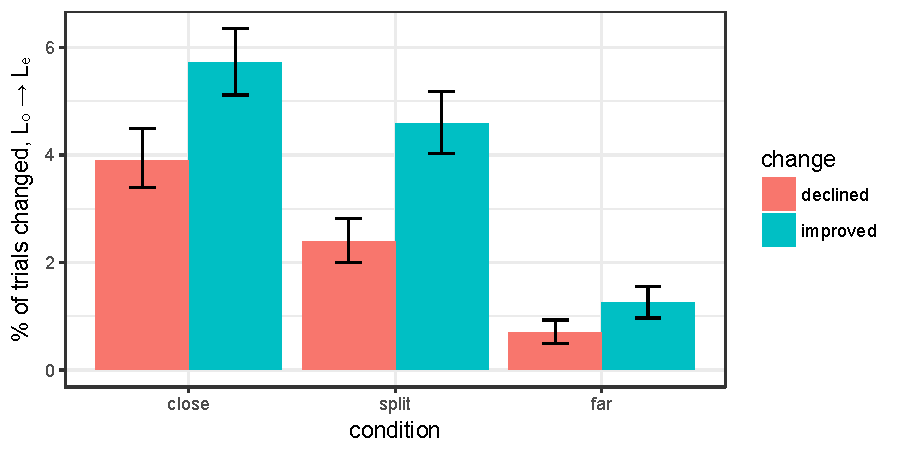
\includegraphics[scale = .45]{figures/changedByCondition.pdf}
\caption{Fraction of examples improved and declined, $\Listener_2$ over $\Listener_0$.}
\label{fig:changedByCondition}
\end{figure}

Breaking out the number of examples changed by condition
(\figref{fig:changedByCondition}) reveals that
the primary gain from the pragmatic model is in the $close$ condition, when the
model has to pick up on the most subtle distinctions.

\begin{figure}
\centering
\todocheck{(give an example of $\Listener^*$ in action here)}
\caption{Conditional probability tables used in the calculation of $\Listener^*$
for one example in the dev set.}
\label{fig:rsaExample}
\end{figure}

Examining the full probability tables for various dev set examples on which
$\Listener^*$ makes a difference reveals a general pattern. In most of these
examples, the alternative utterances sampled from $\Speaker_0$ for one of the
referents $i$ fail to identify
their intended referent to $\Listener_0$. The pragmatic listener interprets
this to mean that referent $i$ is inherently difficult to refer to,
and it compensates by increasing referent $i$'s probability. This is beneficial
when $i$ is the true target but harmful when $i$ is a distractor.

\Figref{fig:rsaExample}
shows one such example: \todocheck{(talk about specific example)}

\subsection{Speaker effectiveness} \label{sec:speaker_eff}

\Tabref{table:speakerVsListener} shows the effectiveness of the two speaker models
(base speaker $\Speaker_0$ and pragmatic speaker $\Speaker_1$) at describing the
target color to the listener models.

The pragmatic speaker is better at communicating
with the listener models, which is unsurprising, because in the case of
$\Listener_0$, the speaker has access to the listener's thought process, and in
the case of $\Listener_2$, the listener has access to the speaker's thought process.

Additionally, however, the listeners are able to understand even $\Speaker_0$'s
utterances better than humans'. This is surprising, because $\Listener_0$ does not
contain an embedded model of either speaker, and $\Listener_2$ uses $\Speaker_0$
only indirectly, as a source of alternative utterances to consider.

\subsection{Tuning the pragmatic parameters} \label{sec:alpha_beta}

As noted in \secref{sec:training}, we use an inverse temperature parameter of
$\alpha = 0.544$ and a base weight of $\beta = -0.15$ for the pragmatic
listener. Particularly surprising is the fact that the optimal value of $\beta$
discovered in grid search is \emph{negative}. This has the effect of amplifying
the difference between $\Listener_0$ and $\Listener_2$: the pragmatic model,
evidently, is not quite pragmatic enough.

The $\alpha$ value of 0.544${}<{}$1 indicates that the pragmatic listener is
modeling a somewhat less reliable speaker than one that uses a straightforward
softmax choice distribution. Various values of $\alpha$ have been shown to
be optimal for different tasks; \todocheck{(citations)}.

\begin{figure}
\centering
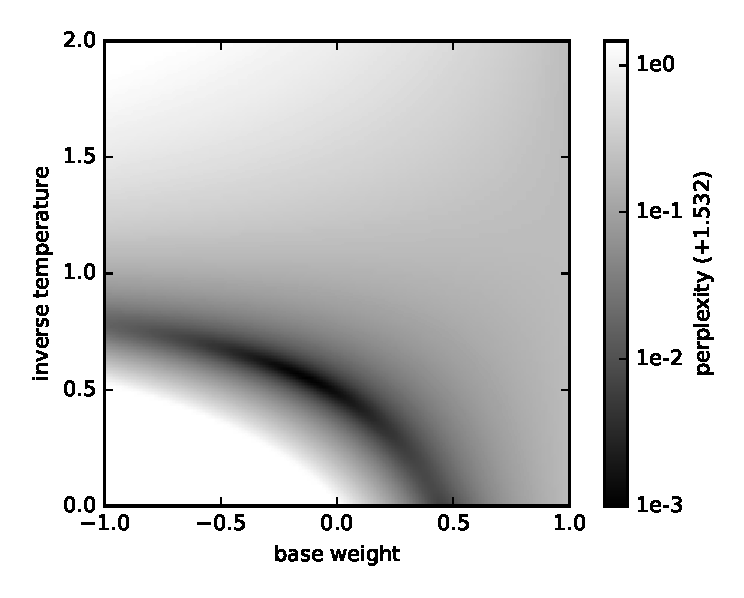
\includegraphics[width=\columnwidth]{figures/alpha_beta.eps}
\caption{Perplexity $\pi$ on tuning set as a function of $\alpha$ and $\beta$, plotted as $\log(\pi - \min_{\alpha,\beta} \pi(\alpha, \beta))$.}
\label{fig:alpha_beta}
\end{figure}

Grid search over values of $\alpha$ and $\beta$ revealed that the optimal values of 
the two parameters are related (\figref{fig:alpha_beta}). Good combinations lay on
a curve with $\alpha$ decreasing as $\beta$ increased; however, negative $\beta$ and
very small $\alpha$ was catastrophic to perplexity.\footnote{We tuned the
parameters on perplexity rather than accuracy because accuracy was noisy and had
many local and global minima.}

\section{Related work}

Prior work combining machine learning with probabilistic pragmatic reasoning
models has largely focused on the speaker side, i.e., generation.
\newcite{Golland2010} develop a pragmatic speaker model,
$\Speaker(\Listener)$, that reasons about log-linear listeners trained on human
utterances containing spatial references in virtual-world environments.
\newcite{Tellex2014a} apply a similar technique, under the name
\term{inverse semantics}, to create a robot that can informatively ask
humans for assistance in accomplishing tasks. \newcite{Monroe2015} implement
an end-to-end trained $\Speaker(\Listener(\Speaker))$ model for referring
expression generation in a reference game task; their model requires enumerating
the set of possible utterances for each context, which is infeasible when
utterances are as varied as those in our dataset.

The closest work to ours that we are aware of is that of
\newcite{AndreasKlein16_NeuralPragmatics}, who also combine neural speaker
and listener models to model pragmatics. They implement and evaluate a
pragmatic speaker $\Speaker(\Listener_0)$, with sampling from a neural
$\Speaker_0$ model to limit the search space and regularize the model toward
human-like utterances.

Our approach goes one step beyond theirs, in that we build a two-level derived
pragmatic model $\Listener(\Speaker(\Listener_0))$; i.e., we use a similar sampling
scheme to limit the search space in speaker modeling, and then explicitly normalize
over the colors in the context to derive a pragmatic listener.

Additionally, we use more powerful recurrent models for both the base speaker and the
base listener; \newcite{AndreasKlein16_NeuralPragmatics} use multi-layer perceptron
models over $n$-gram features. We also include the $\alpha$ inverse temperature
parameter from \newcite{Goodman2013}, and we use a different strategy for blending the
pragmatic and base models: their model blends the base speaker and base listener
$\Speaker_0^{\beta} \cdot \Listener_0^{\beta}$ and
normalizes across utterances to implicitly define a different pragmatic model,
whereas we first compute the full normalized pragmatic
model $\Listener(\Speaker(\Listener_0))$ and blend it with a base listener by
$\Listener_0^{\beta} \cdot \Listener(\Speaker(\Listener_0))^{1 - \beta}$.

\section{Conclusion}

In this paper we presented a newly-collected corpus of color descriptions from
reference games, and we showed that combining a model of pragmatic reasoning
with a neural color description understanding model results in more accurate
context-dependent description understanding compared with the neural model alone.

It is reasonable to expect that a model trained in an end-to-end fashion on
pragmatic data would be preferable to a pragmatic reasoning scheme applied on
top of a pre-trained base model.
Indeed, the probabilistic pragmatic work in the cognitive science literature
on which this work is based assumes the base listener represents literal semantics
and is not pragmatic at all; this suggests that our model relies on the base
listener failing to learn pragmatic behavior already present in the dataset.
An enticing avenue of future work is to use variational methods to scale
up an end-to-end pragmatic model like that of \newcite{Monroe2015} to
allow for arbitrarily large spaces of alternative utterances.
\todocheck{(todo: more wrap-up?)}

%\section{Credits}
%
%This document has been adapted from the instructions for ACL proceedings, including those for ACL-2008 by Johanna D. Moore, Simone Teufel, James Allan, and Sadaoki Furui, those for ACL-2005 by Hwee Tou Ng and Kemal Oflazer, those for ACL-2002 by Eugene Charniak and Dekang Lin, and earlier ACL and EACL formats. Those versions were written by several people, including John Chen, Henry S. Thompson and Donald Walker. Additional elements were taken from the formatting instructions of the {\em International Joint Conference on Artificial Intelligence}.
%
%\section{Introduction}
%
%The following instructions are directed to authors of papers submitted to TACL or accepted for publication. All authors are required to adhere to these specifications. Authors are required to provide a Portable Document Format (PDF)
%% das: removed reference to PostScript
%% and PostScript
%version of their papers. \textbf{The proceedings will be printed on
%US-Letter paper}. Authors from countries in which access to
%word-processing systems is limited should contact TACL editors at editors-in-chief@transacl.org as soon as possible.
%
%
%\section{General Instructions}
%
%Manuscripts must be in two-column format. Exceptions to the two-column format include the title,
%authors' names and complete addresses, which must be centered at the top of the first page,
%and any full-width figures or tables (see the guidelines in Subsection~\ref{ssec:first}). {\bf Type single-spaced}.
%Start all pages directly under the top margin. See the guide-lines later regarding formatting the first page. Do not number the pages.
%
%\subsection{Electronically-available resources}
%
%TACL provides this description in \LaTeX2e (tacl.tex) and PDF format (tacl.pdf), along with the LATEX2e style file used to format it (acl2012.sty) and an ACL bibliography style (acl2012.bst).  A Microsoft Word template file (tacl.dot) is also available. We require the use of these style files, which have been appropriately tailored for TACL. If you have an option, we recommend that you use the \LaTeX2e version. \textbf{If you will be using the Microsoft Word template, we suggest that you anonymize your source file so that the pdf produced does not retain your identity.} This can be done by removing any personal information from your source
%document properties.
%
%
%\subsection{Format of Electronic Manuscript}
%\label{sect:pdf}
%
%For the production of the electronic manuscript you must use Adobe's
%Portable Document Format (PDF). This format can be generated from
%postscript files: on Linux/Unix systems, you can use {\tt ps2pdf} for this
%purpose; under Microsoft Windows, you can use Adobe's Distiller, or
%if you have {\tt cygwin} installed, you can use {\tt dvipdf} or
%{\tt ps2pdf}.  Note
%that some word processing programs generate PDF which may not include
%all the necessary fonts (esp. tree diagrams, symbols). When you print
%or create the PDF file, there is usually an option in your printer
%setup to include none, all or just non-standard fonts.  Please make
%sure that you select the option of including ALL the fonts.  {\em Before sending it, test your PDF by printing it from a computer different from the one where it was created}. Moreover,
%some word processor may generate very large postscript/PDF files,
%where each page is rendered as an image. Such images may reproduce
%poorly.  In this case, try alternative ways to obtain the postscript
%and/or PDF.  One way on some systems is to install a driver for a
%postscript printer, send your document to the printer specifying
%``Output to a file'', then convert the file to PDF.
%
%Additionally, it is of utmost importance to specify the {\bf US-Letter format} (8.5in $\times$ 11in) when formatting the paper. When working with {\tt dvips}, for instance, one should specify {\tt -t letter}.
%
%Print-outs of the PDF file on US-Letter paper should be identical to the
%hardcopy version.  If you cannot meet the above requirements about the
%production of your electronic submission, please contact the
%publication chair above as soon as possible.
%
%
%\subsection{Layout}
%\label{ssec:layout}
%
%Format manuscripts two columns to a page, in the manner these
%instructions are formatted. The exact dimensions for a page on US-letter
%paper are:
%
%\begin{itemize}
%\item Left and right margins: 1in
%\item Top margin:1in
%\item Bottom margin: 1in
%\item Column width: 3.15in
%\item Column height: 9in
%\item Gap between columns: 0.2in
%\end{itemize}
%
%\noindent Papers should not be submitted on any other paper size. If you cannot meet the above requirements about the production of your electronic submission, please contact the publication chair above as soon as possible.
%
%\subsection{Fonts}
%
%For reasons of uniformity, Adobe's {\bf Times Roman} font should be
%used. In \LaTeX2e{} this is accomplished by putting
%
%\begin{quote}
%\begin{verbatim}
%\usepackage{times}
%\usepackage{latexsym}
%\end{verbatim}
%\end{quote}
%in the preamble. If Times Roman is unavailable, use {\bf Computer
%Modern Roman} (\LaTeX2e{}'s default).  Note that the latter is about
%10\% less dense than Adobe's Times Roman font.
%
%
%\begin{table}[h]
%\begin{center}
%\begin{tabular}{|l|rl|}
%\hline \bf Type of Text & \bf Font Size & \bf Style \\ \hline
%paper title & 15 pt & bold \\
%author names & 12 pt & bold \\
%author affiliation & 12 pt & \\
%the word ``Abstract'' & 12 pt & bold \\
%section titles & 12 pt & bold \\
%document text & 11 pt  &\\
%captions & 10 pt & \\
%abstract text & 10 pt & \\
%bibliography & 10 pt & \\
%footnotes & 9 pt & \\
%\hline
%\end{tabular}
%\end{center}
%\caption{\label{font-table} Font guide. }
%\end{table}
%
%\subsection{The First Page}
%\label{ssec:first}
%
%Center the title, author's name(s) and affiliation(s) across both
%columns. Do not use footnotes for affiliations.  Do not include the
%paper ID number assigned during the submission process.
%Use the two-column format only when you begin the abstract.
%
%{\bf Title}: Place the title centered at the top of the first page, in
%a 15 point bold font.  (For a complete guide to font sizes and styles, see Table~\ref{font-table}.)
%Long title should be typed on two lines without
%a blank line intervening. Approximately, put the title at 1in from the
%top of the page, followed by a blank line, then the author's names(s),
%and the affiliation on the following line.  Do not use only initials
%for given names (middle initials are allowed). Do not format surnames
%in all capitals (e.g., ``Zhou,'' not ``ZHOU'').  The affiliation should
%contain the author's complete address, and if possible an electronic
%mail address. Leave about 0.75in between the affiliation and the body
%of the first page. The title, author names and addresses should be completely identical to those entered to the electronic paper submission website in order to maintain the consistency of author information among all publications of the conference.
%
%{\bf Abstract}: Type the abstract at the beginning of the first
%column.  The width of the abstract text should be smaller than the
%width of the columns for the text in the body of the paper by about
%0.25in on each side.  Center the word {\bf Abstract} in a 12 point
%bold font above the body of the abstract. The abstract should be a
%concise summary of the general thesis and conclusions of the paper.
%It should be no longer than 200 words. The abstract text should be in 10 point font.
%
%{\bf Text}: Begin typing the main body of the text immediately after
%the abstract, observing the two-column format as shown in
%the present document. Do not include page numbers.
%
%{\bf Indent} when starting a new paragraph. For reasons of uniformity,
%use Adobe's {\bf Times Roman} fonts, with 11 points for text and
%subsection headings, 12 points for section headings and 15 points for
%the title.  If Times Roman is unavailable, use {\bf Computer Modern
%Roman} (\LaTeX2e's default; see section \ref{sect:pdf} above).
%Note that the latter is about 10\% less dense than Adobe's Times Roman
%font.
%
%\subsection{Sections}
%
%{\bf Headings}: Type and label section and subsection headings in the
%style shown on the present document.  Use numbered sections (Arabic
%numerals) in order to facilitate cross references. Number subsections
%with the section number and the subsection number separated by a dot,
%in Arabic numerals. Do not number subsubsections.
%
%{\bf Citations}: Citations within the text appear
%in parentheses as~\cite{Gusfield:97} or, if the author's name appears in
%the text itself, as Gusfield~\shortcite{Gusfield:97}. Append lowercase letters to the year in cases of ambiguities. Treat double authors as in~\cite{Aho:72}, but write as in~\cite{Chandra:81} when more than two authors are involved. Collapse multiple citations as in~\cite{Gusfield:97,Aho:72}. Also refrain from using full citations as sentence constituents. We suggest that instead of
%\begin{quote}
%``\cite{Gusfield:97} showed that ...''
%\end{quote}
%you use
%\begin{quote}
%``Gusfield \shortcite{Gusfield:97}   showed that ...''
%\end{quote}
%
%If you are using the provided \LaTeX{} and Bib\TeX{} style files, you
%can use the command \verb|\newcite| to get ``author (year)'' citations.
%
%As reviewing will be double-blind (except that action editors know author identity and authors know action-editor identity), the submitted version of the papers should not include the
%authors' names and affiliations. Furthermore, self-references that
%reveal the author's identity, e.g.,
%\begin{quote}
%``We previously showed \cite{Gusfield:97} ...''
%\end{quote}
%should be avoided. Instead, use citations such as
%\begin{quote}
%``Gusfield \shortcite{Gusfield:97}
%previously showed ... ''
%\end{quote}
%
%To be clear: You should reference your prior work if it is relevant; but use the third person instead of the 1st person and in place of references like “(Anonymous) showed…”, since such anonymized references do not allow readers to examine relevant related work.
%
%Authors’ names should also be removed from the ``Document Properties'' display that can be viewed using Adobe Acrobat’s ``File $\rightarrow$ Properties'' menu.
%
%Please do not include acknowledgements when submitting your papers. Papers that do not conform
%to these requirements may be rejected without review.
%
%\textbf{References}: Gather the full set of references together under
%the heading {\bf References}; place the section before any Appendices,
%unless they contain references. Arrange the references alphabetically
%by first author, rather than by order of occurrence in the text.
%Provide as complete a citation as possible, using a consistent format,
%such as the one for {\em Computational Linguistics\/} or the one in the
%{\em Publication Manual of the American
%Psychological Association\/}~\cite{APA:83}.  Use of full names for
%authors rather than initials is preferred.  A list of abbreviations
%for common computer science journals can be found in the ACM
%{\em Computing Reviews\/}~\cite{ACM:83}.
%
%The \LaTeX{} and Bib\TeX{} style files provided roughly fit the
%American Psychological Association format, allowing regular citations,
%short citations and multiple citations as described above.
%
%{\bf Appendices}: Appendices, if any, directly follow the text and the
%references (but see above).  Letter them in sequence and provide an
%informative title: {\bf Appendix A. Title of Appendix}.
%
%\textbf{Acknowledgment} sections should go as a last section immediately
%before the references. Do not number the acknowledgement section.
%
%\subsection{Footnotes}
%
%{\bf Footnotes}: Put footnotes at the bottom of the page. They may
%be numbered or referred to by asterisks or other
%symbols.\footnote{This is how a footnote should appear.} Footnotes
%should be separated from the text by a line.\footnote{Note the
%line separating the footnotes from the text.}  Footnotes should be in 9 point font.
%
%\subsection{Graphics}
%
%{\bf Illustrations}: Place figures, tables, and photographs in the
%paper near where they are first discussed, rather than at the end, if
%possible.  Wide illustrations may run across both columns and should be placed at
%the top of a page. Color illustrations are discouraged, unless you have verified that
%they will be understandable when printed in black ink.
%
%{\bf Captions}: Provide a caption for every illustration; number each one
%sequentially in the form:  ``Figure 1. Caption of the Figure.'' ``Table 1.
%Caption of the Table.''  Type the captions of the figures and
%tables below the body, using 10 point text.
%
%\section{Translation of non-English Terms}
%
%It is also advised to supplement non-English characters and terms
%with appropriate transliterations and/or translations
%since not all readers understand all such characters and terms.
%
%Inline transliteration or translation can be represented in
%the order of: original-form transliteration ``translation''.
%
%\section{Length of Submission}
%\label{sec:length}
%
%Submissions may consist of seven to ten (7-10) letter format (not A4) pages of content and unlimited additional pages (only) allowed for references. Papers that are revisions of submissions with prior (b) or (c) decisions may be allowed one to two additional pages of content to accommodate required revisions.
%
%Appendices (if any) are counted as content pages. Papers that do not conform to the specified length and
%formatting requirements are subject to re-submission.
%
%
%\section*{Acknowledgments}
%
%Do not number the acknowledgment section. Do not include this section when submitting your paper for review.

\bibliography{colors}
\bibliographystyle{acl2012.bst}

\end{document}



